\subsection{CU12 Modificar Empleado}
Al momento de seleccionar un registro de la pantalla de 'Visualizar Empleados' (figura \ref{fig:Pantalla Visualizar Empleados - Vista de Escenarios}) y seleccionar la opción de modificar el registro del empleado, se mostrará la ventana de modificación, la cual contiene un formulario de actualización de los datos. Cada uno de los campos estará lleno con la información que esta guardada dentro de la base de datos. El administrador podrá modificar dicha información y podrá seleccionar alguno de los botones de la parte inferior de la pantalla:
\begin{itemize}
	\item \textbf{Modificar:} Al dar click en esta opción, el sistema valida si toda la información es correcta (formato, estructura y si los campos están llenos). En caso de que no sea así, el sistema mostrará una alerta (figura \ref{fig:Alerta Modificar Empleado - Vista de Escenarios}).
	\item \textbf{Cancelar:} Salir de esa ventana y regresar a al pantalla anterior. (Figura \ref{fig:Pantalla Visualizar Empleados - Vista de Escenarios}).
\end{itemize}
\begin{figure}[!h]
	\centering
	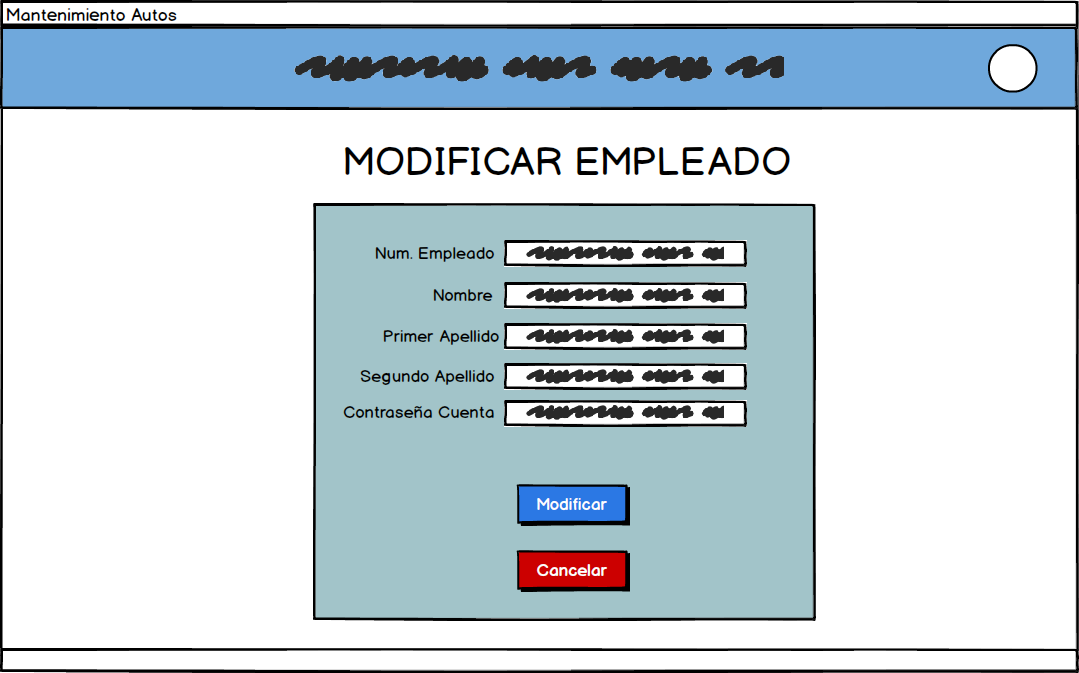
\includegraphics[width=0.8\textwidth]{./diseno/vescenarios/imagenes/modificarEmpleado}
	\caption{Pantalla Modificar Empleado - Vista de Escenarios}
	\label{fig:Pantalla Modificar Empleado - Vista de Escenarios}
\end{figure}
\begin{figure}[!h]
	\centering
	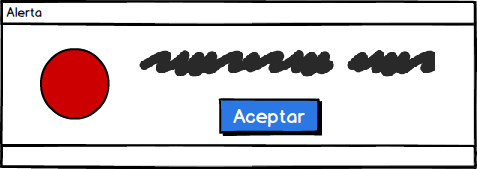
\includegraphics[width=0.3\textwidth]{./diseno/vescenarios/imagenes/alerta}
	\caption{Alerta Modificar Empleado - Vista de Escenarios}
	\label{fig:Alerta Modificar Empleado - Vista de Escenarios}
\end{figure}
\clearpage